\chapter{Data Science and Learning Basics}\label{ch_data_science}
\chapterauthor{Jeff Yoshimi}

% Discussion of tensors needs to be centralized. Current SupervisedFF has the main discussion. There is a footnote here right now.

In this chapter, we cover fundamental concepts used when training neural networks, focusing in particular on the tables of data involved. Tables of data are the bread and butter of any neural network practitioner, and we must understand them well.  Thus, in this chapter we begin with a brief introduction to \glossary{data science}, which is an area of practice focused on processing and analyzing datasets, often using machine learning models. Though data science is most connected with engineering uses of neural networks (see section \extref{typesOfResearch}), concepts from this field are equally applicable any time neural network models are used. Moreover, anyone who uses neural networks in practice must understand how to deal with data: how to clean it up, re-code certain features, produce exploratory visualizations, and so forth. In this chapter, we begin with an overview of basic concepts from data science. At the end of the chapter, we use these concepts to differentiate the main types of learning algorithm in neural networks.

\section{Data Science Workflow}

Here is a basic workflow that is common in data science:

\begin{enumerate}
\item Getting the data. Describing it. Understanding its basic features. Coming up with useful column names or ``feature'' names. You might obtain data from an experiment, download data from a website, or be given a large table or spreadsheet. To get a better sense of the nature of the data used in a neural network, and the kinds of work needed to wrangle it into a format that a network can process, several public repositories of machine learning and other kinds of data exist.\footnote{See: \url{https://archive.ics.uci.edu/ml/index.php} and \url{https://en.wikipedia.org/wiki/List_of_datasets_for_machine_learning_research}. Many other sources of data exist, of course, including US Census data, World Health organization data, etc. The website Kaggle has a large repository of datasets and machine learning tasks that can be pursued in a game-like competitive framework. Many public tools, like R, sklearn, Pytorch, and Tensorflow have datasets included.}  Special issues arise when using the very large datasets (``big data'') required to effectively train some machine learning models\footnote{Cf. \url{https://en.wikipedia.org/wiki/Big_data} and ETL \url{https://en.wikipedia.org/wiki/Extract,_transform,_load}.}, but we will focus on small datasets that are useful for illustrative purposes. 
\item Visualizing the data / Exploratory Data Analysis (EDA). Developing an initial feel for  data, often using visualizations.\footnote{See \url{https://en.wikipedia.org/wiki/Exploratory_data_analysis}.} Creating pictures that illustrate the main features of your data, which suggest how your machine learning task might be solved, e.g. finding data that show a correlation between some input data and the target data.
\item Preparing the data. Also called data wrangling. Creating useful features. Filling in missing data. Removing outliers. Discussed in more detail in section \ref{wrangling}.
\item Create and train a model. Choose a type of model and then train it. This is where  neural networks come in. In machine learning there are many kinds models, like multiple regression and decision trees and ensembles of models. But we focus on neural networks.
\item Assessing the model's performance on test data. We will see that it is often important to first train a model on one set of data, and then to validate the model on a separate set of data.
\end{enumerate}

We will not discuss obtaining data or exploratory data analysis here. We discuss data wrangling in section \ref{wrangling}. The rest of the chapter, and much of the rest of the book, is focused on creating and training neural network models. Assessing performance is briefly discussed in several places in this chapter and the next few chapters.

Of these steps, the main one in terms of learning is the step where we build and train a model. When the model is trained, we update its \glossary{parameter}s. Parameters are discussed further in the dynamical systems chapter, chapter \extref{ch_dst}. In a neural network, these parameters are usually weights and biases (chapter \extref{ch_act_functions}). Parameters change the dynamics of a dynamical system. For a recurrent network, that means they change what activation patterns occur over time. They change a phase portrait. For a feed-forward network, they change the input-output function the network produces. Feed-forward networks take an input vector and produce an output vector. The process of training a feed-forward network is the process of modifying the parameters in such  a way as to change the vector-valued function it implements. In chapter \extref{ch_supervised}, we see how to update the parameters of a feed-forward network to achieve a desired input-output function, e.g. to make a network, which recognizes letters or faces in images. In chapter \extref{ch_supervised_recurrent}, we see how the parameters of a recurrent network can be trained to achieve desired dynamics. This type of network can be used to produce realistic speech and convincing text, as we will see.
% Ref to vector valued function. Reverse FF and recurrent?

However, in this chapter we also see all the other work that is involved in actually building a neural network model. Data must be gathered, analyzed, and cleaned up. And then we must partition our data in a special way in order to test how well it works not just on the data we trained it on, but also on new data it has never seen before.\footnote{A worked example illustrating many of the ideas in this chapter in tensor flow is here: \url{https://www.youtube.com/watch?v=-vHQub0NXI4}.}

\section{Datasets}

As discussed in chapter \extref{ch_intro}, neural networks are usually linked to an \emph{environment}, where that environment is often a simple table or spreadsheet. Even though we are just dealing with tables here, there are a lot of concepts and terms to master. We will take a  \glossary{dataset} to be a table of values to be used by a neural network. A row of a dataset is an \glossary{example}, \emph{instance}, or \emph{case}. A column of a dataset is a \glossary{feature} or \emph{attribute}. The columns of a dataset often correspond to the nodes of a network. Rows often correspond to inputs that will be sent to the input layer of a network, or used to describe desired outputs. These rows and columns can be transformed, partitioned, and manipulated in various ways, as we will see. 
% Other usages. Haykin uses "sample" for the entire training set. He also says: ``Random variables: Italic uppercase symbols are used for random variables.The sample value (i.e., one-shot realization) of a random variable is denoted by the corresponding italic lowercase symbol. For example, we write X for a random variable and x for its sample value.''   Deep learning book uses ``example''. Fausett using training sample sometimes. UCI Machine learning uses instances and attributesI, n psychology  rows are sometimes called ``subjects'' or ``items'', and columsn are covariates or variables. 
% Training sample is common, but a whole dataset is often a sample in the statistical sense, so it's confusing.
% Datasets have _distributions_ associated with them. EDA.
  
As an example, consider the Motor Trend Cars dataset  (``\emph{mtcars}''),  shown in Fig. \ref{cars_dataset}, which is included with the R statistical computing environment. The data is based on a 1974 issue of the car magazine \emph{Motor Trend}, which road-tested about 30 models of cars in the 1973-74 model year and measured a range of performance features.\footnote{See \url{https://stat.ethz.ch/R-manual/R-devel/library/datasets/html/mtcars.html}. A neural network that processes this dataset is included with Simbrain as a script called \emph{backprop\_cars.bsh}. } The dataset contains 30 examples with 10 features each, 6 of which are shown (the row indices and the model names will not be sent to any neural network, so we don't count them as features). Notice that this table, as it stands, is not ready to be used by a neural network. The neural network can't deal with the names (which are strings, rather than numbers), and as we'll see, some of the values (like horsepower) are kind of big for a node that is only meant to deal with small numbers between -1 and 1. However, after a bit of processing, the data can be used to train a neural network to, for example, predict the fuel efficiency of a car based on its weight and number of cylinders.\footnote{A detailed discussion of this case is here: \url{https://www.youtube.com/watch?v=K4GZ51cozRs}.}

% Include code for this in image_masters
\begin{figure}[h]
\centering
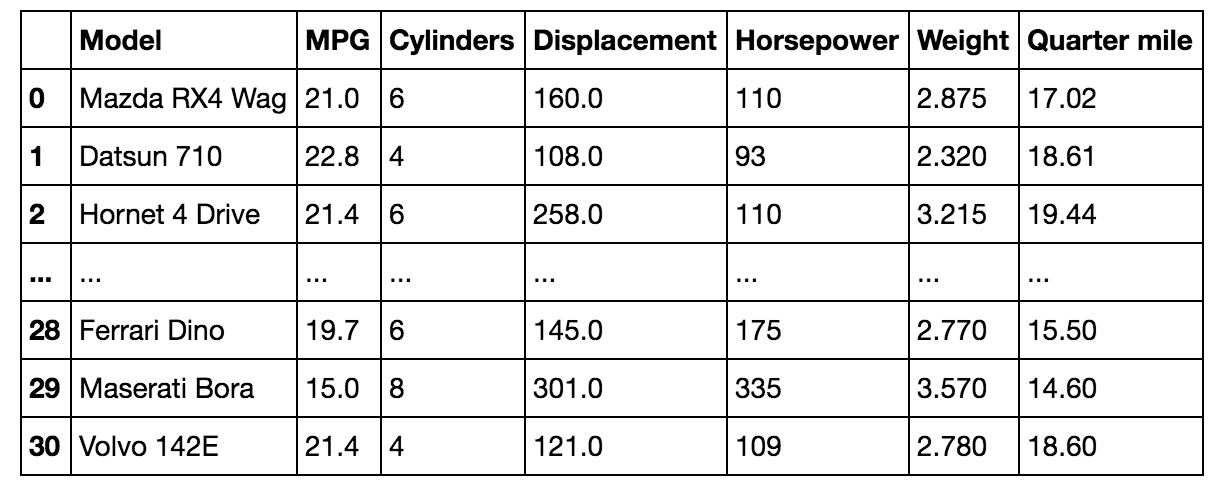
\includegraphics[scale=0.6]{./images/CarsBase.png}
\caption[Screenshot of the Motor Trend Car Road Tests dataset included with R.]{A fragment of  the \emph {mtcars} dataset showing some of its examples (rows) and some of its features (columns) }
\label{cars_dataset}
\end{figure}

We can distinguish two main types of data, beginning with \glossary{categorical data}, also known as ``nominal data''. Categorical data can take one of a discrete list of values. For example, cards can have one of four suits: hearts, diamonds, spades, or aces. The state one lives in can be one of 50 values. In the example in  Figure \ref{cars_dataset}, cylinders appears to be categorical, because there are three possible values for that feature: 4, 6, or 8 cylinders. For a neural network, these will be converted to numerical data using a ``one-hot-encoding'', as we will see. 

Second, \glossary{numerical data} is data that is already in the form of numbers. These numbers can either be real-valued (represented by floating point values in a computer) or integer-valued. Examples: age, income, house prices, hours of study, GPA, length, width, weight, caloric intake. In Figure \ref{cars_dataset}, most of the columns are numerical. A few seem to be integers (displacement, horsepower), and others are clearly real-valued (weight, quarter-mile).\footnote{ In more rigorous treatments (derived from the study of scale types in measurement theory), ordinal, interval, and ratio scales are distinguished. We collapse interval and rational scales into numerical. Ordinal data (e..g first, second, and third in line) can often be treated as integers or using a one-hot encoding.}

To get a general sense of how datasets are used with neural networks, see Fig \ref{data_inputs}. Each column, each feature, is generally associated with the nodes of a network. The figure shows an input dataset, but we will see there are other types of datasets used with neural networks as well.

\begin{figure}[h]
\centering
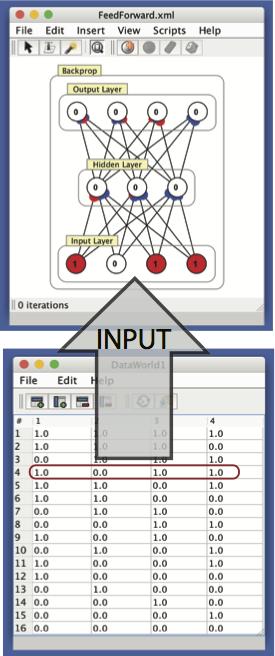
\includegraphics[scale=.9]{./images/dataset_inputs.png}
\caption[Simbrain screenshot with graphical elements added by Pamela Payne.]{An example of an input dataset, which illustrates one standard way datasets are used with neural networks. Each row of the dataset is thought of as one input vector for the neural network.}
\label{data_inputs}
\end{figure}

\section{Data Wrangling (or Preprocessing)}\label{wrangling}
% Possibly expand feature engineering into a new section
% Word embedding should itself be its own discussion, with forward refs to Supervised recurrent. The importance of representing words with a similarity space.

Raw data isn't usually ready to be fed to a neural network. Sometimes a dataset contains strings of text, images, sound files, and other structures that must be converted into a numerical format. Neural networks want \emph{numbers}, and they often want those numbers to be a certain way. So we have to pre-process the data in various ways. Our ultimate goal is typically to have a table all of whose cells contain numbers that lie within a fairly small range, like between -1 and 1 or between 0 and 1.\footnote{At that point our dataset has the form of a matrix (cf. Chapter \extref{ch_linear_algebra}), and mathematical operations of linear algebra can be applied to it.} That is, we want to end up with a dataset where each row is an input vector that can be fed to the input nodes of a neural network.

So we have work to do. We have to convert non-numerical data to single numbers. We have to fill in missing data. And even when all the data is numerical we must often do further things like rescaling the data. These operations correspond to \glossary{pre-processing} the data. This is sometimes called \glossary{data wrangling} or ``data munging''.\footnote{For a sense of some of the ways data can be wrangled, have a look at the \emph{scikit-learn} pre-processing library: \url{http://scikit-learn.org/stable/modules/preprocessing.html}.}  Here is how wikipedia defines it:

\begin{quotation}
Data munging or data wrangling is loosely defined as the process of manually converting or mapping data from one `raw' form into another format that allows for more convenient consumption of the data with the help of semi-automated tools.\footnote{\url{https://en.wikipedia.org/wiki/Data_wrangling}.} 
\end{quotation}

The process of wrangling data is usually understood as a step-wise workflow or pipeline, where the data is obtained and transformed in stages until it is ready to be processed by a neural network. There are different ways  of understanding this workflow. Here is a generic version of a data wrangling workflow:
\begin{itemize}
\item Data cleaning: remove, fix, or otherwise deal with bad data. Fill in missing data.
\item Feature-extraction and feature-engineering: Transform data (e.g. text, images, audio files, DNA sequences) into a numerical format and more generally produce a set of numerical features to be used by the neural network.
\item Rescaling: alter the numbers in the dataset to, for example, ensure that they are all in the range $(-1,1)$
\end{itemize}

The first step is \glossary{data cleaning} or ``data cleansing''. There might be stray characters that make it hard to import the data, or columns that are irrelevant to what you are trying to do. Often it helps to simply focus on a subset of columns or rows (\emph{subsetting}). A related cleansing step is dealing with missing data, using methods of \emph{data imputation} to determine a policy for filling in missing data. Common techniques include filling in these cells  with 0's, or with the mean value of the column they are in.\footnote{See \url{https://towardsdatascience.com/how-to-handle-missing-data-8646b18db0d4} and \url{http://www.stat.columbia.edu/~gelman/arm/missing.pdf}.}

The next step, \glossary{feature-extraction}  involves converting non-numeric data into a numerical form suitable for a neural network. Images, movies, audio, DNA sequences, and of course, text, are all non-numeric data that must be converted to a numerical format.\footnote{Also see \url{http://scikit-learn.org/stable/modules/feature_extraction.html}} This is often the most involved and  most important step in building a working model. Many of the earliest connectionist models (e.g. Nettalk) relied on clever ways of representing written and spoken speech in a vectorized way that could be fed to a network.

We are construing this step quite broadly to include any steps involved in coming up with features (numerical columns) for a dataset, from flattening a matrix, to combining features into new features. The latter is sometimes also called \emph{feature-engineering}, where a new feature is designed for use in training a model, e.g. deciding not to feed a neural network height and width information separately, but rather to feed it the ratio of the height to the width of an image, which might yield better results for some applications. Another example in the \emph{mtcars} dataset would be to take the model of a car and then consult a database online to find new features of the cars.\footnote{In competitive machine learning, as in Kaggle, often the best solutions are based on clever feature engineering, more so than anything in the machine learning model itself.}

% Time, date as features, which raise special issues
% Acoustic features is itself a cog-sci discussion. So this overlaps cog-sci. See Magnuson talk.
% Work more on the feature discussion in relation to deep learning, which is basically a massive feature detector pre-pended to a standard 3 layer ff network.
Here are some examples of feature extraction in this fairly broad sense. 
\begin{itemize}
\item Taking a feature like the model of a car, state of residence, or gender, and converting it into a vector of binary values. There are several ways to do this, but the most common is using a \glossary{One-hot} or ``one-of-$k$'' encoding, which is a type of coding that converts categorical data to binary vectors.\footnote{See \url{https://en.wikipedia.org/wiki/One-hot}.} If we have three categories--Fish, Swiss, and Gouda--then we can use a one-of-three encoding to represent Fish as $(1,0,0)$, Swiss as $(0,1,0)$, and Gouda as $(0,0,1)$. In a bank of nodes, this corresponds to one node being active (``hot'') and the other nodes being inactive, hence ``one-hot'' encoding. One is hot, and the other is not. For example, in the cars dataset, we can represent 4-cylinder, 6-cylinder, and 8-cylinder by a one-hot (in this case one-of-3) encoding, as in Fig. \ref{cars_onehot}. Notice that the cylinder column in Fig. \ref{cars_dataset} has been  replaced by three columns. The column that has a ``1'' in it indicates whether the car is 4, 6, or 8 cylinders. These are also called dummy or indicator variables in psychology. They are also a form of localist as contrasted with distributed representation (see chapter \extref{ch_intro}).
\item Taking a matrix and ``flattening'' it into a vector that can be treated as a row of a dataset. This is often done with images. Sometimes an even more complex object, a \emph{tensor}, must be flattened.\footnote{A tensor is like a generalized matrix, a multi-dimensional array. A vector is a rank 1 tensor, a matrix is a rank 2 tensor, a set of matrices is a rank 3 tensor, a rank 4 tensor is a set of these sets, etc. See \url{https://en.wikipedia.org/wiki/Tensor}.}  Color images are often represented as three separate pixel  images, corresponding to red, green, and blue channels. So we have three matrices that must be flattened and concatenated to produce one long vector, which is then a proper row of a dataset that can be fed to a network.
\item Converting strings of texts to vectors. Thus, the word ``red'' might become the vector $(1,0,1,0,1,1)$. Techniques for converting linguistic data to vectors are sometimes referred to as methods of \emph{word embedding}. Word embedding is a major area of research in its own right.\footnote{See \url{https://en.wikipedia.org/wiki/Word_embedding}. A famous algorithm for word embedding is word2vec. See \url{https://www.tensorflow.org/tutorials/word2vec}.}
\item Dividing a sound file into smaller time windows and converting those ``clips'' of audio into vectors, often using signal processing techniques like Fourier analysis.
\item Hand coding video or audio data in some way, e.g. counting how many times a participant in a videotaped experiment hits a doll, or how many questions a participant asks. This kind of technique is often used in experimental settings, e.g. in psychology.\footnote{See \url{https://en.wikipedia.org/wiki/Coding_(social_sciences)}.}
\end{itemize}
% Representation / representation learning from deep learning book. How data is represented is the first step in a machine learning 
% Chris Kello quote. ``It all depends on your representation. You win or lose based on that.''
% E.g. the old https://en.wikipedia.org/wiki/Wickelphone stuff
% Tensor footnote redundant with deep nets. Consolidate
% Positional encodings in transfers is a nice case of feature engineering, because it allowed an entirely new architecture: a way to allow sequential inputs to recurrent networks to be replaced by parallel inputs, by tagging vector embedded tokens with positional information.

\begin{figure}[h]
\centering
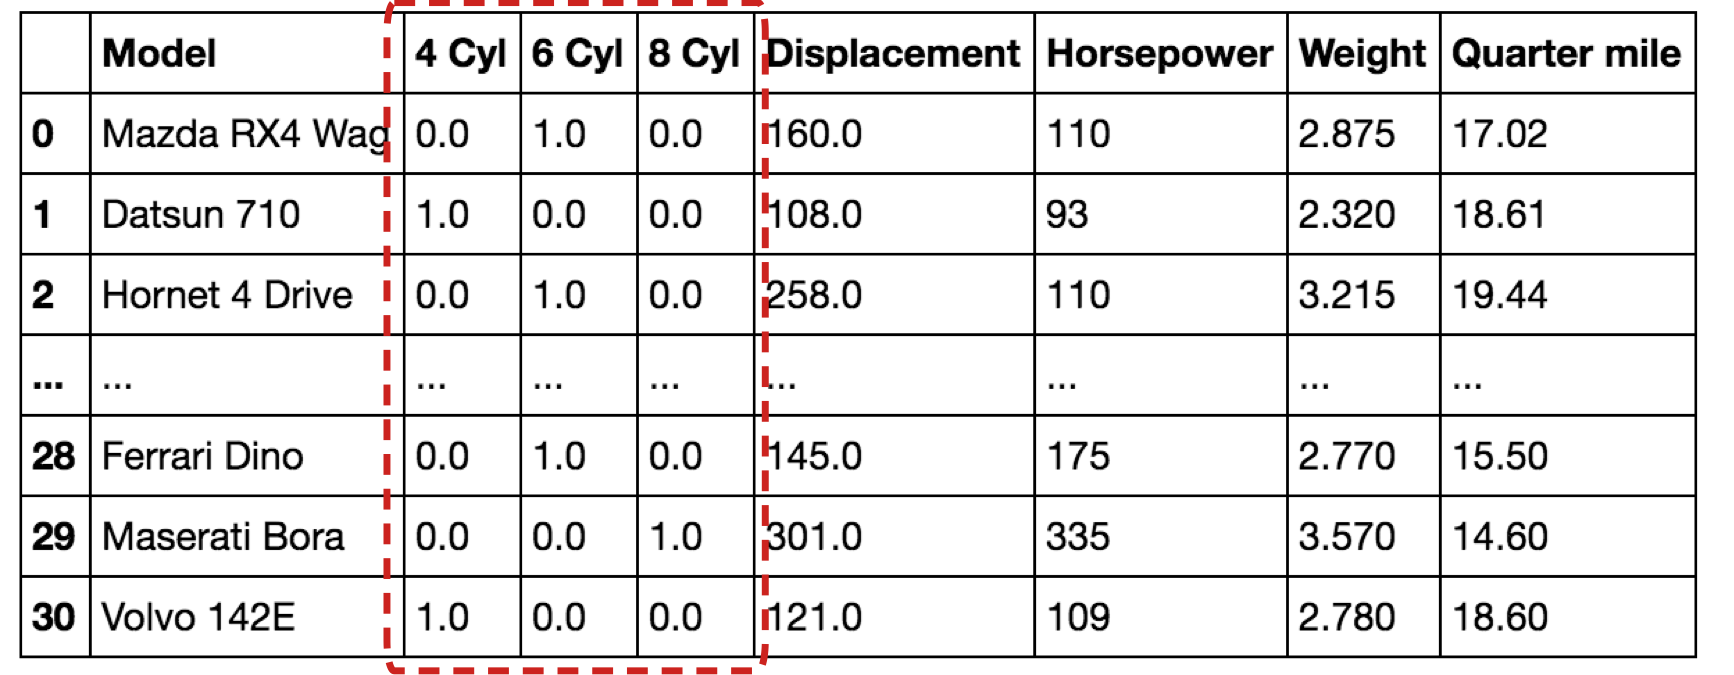
\includegraphics[height=50mm]{./images/CarsOneHot.png}
\caption[Screenshot of the Motor Trend Car Road Tests dataset included in R.]{Convert cylinders to a binary ``one-hot'' encoding.}
\label{cars_onehot}
\end{figure}

Having coded all data as numerical, additional work often remains to be done, in particular, \glossary{rescaling} the data so that they fit in some standard range, e.g. $(0,1)$ or $(-1,1)$. Figure \ref{cars_dataset_scaled} shows the \emph{mtcars} dataset of figure \ref{cars_onehot} after all columns have been rescaled to lie between 0 and 1. A simple and common way to do this for positive valued data is to divide each entry by the maximum value in that column. A similar method works on data that contains negative values. This is sometimes called \emph{min-max scaling}.\footnote{It can also be called ``normalization'' but that term is confusing because it is used in linear algebra in a slightly different way.} This method ensures that all data are in the range  $(0,1)$. Another method is standardizing, where each value in a column is centered at the mean and scaled by standard deviation. This makes it intuitive to interpret data. If we standardize a column, then the 0's correspond to average values, positive values are above average, and negative values are below average (in statistics this is sometimes called a $z$-score). Anything above 1 is unusually large, and similarly for values below -1. However, this method allows values above 1 and below -1. 

\begin{figure}[h]
\centering
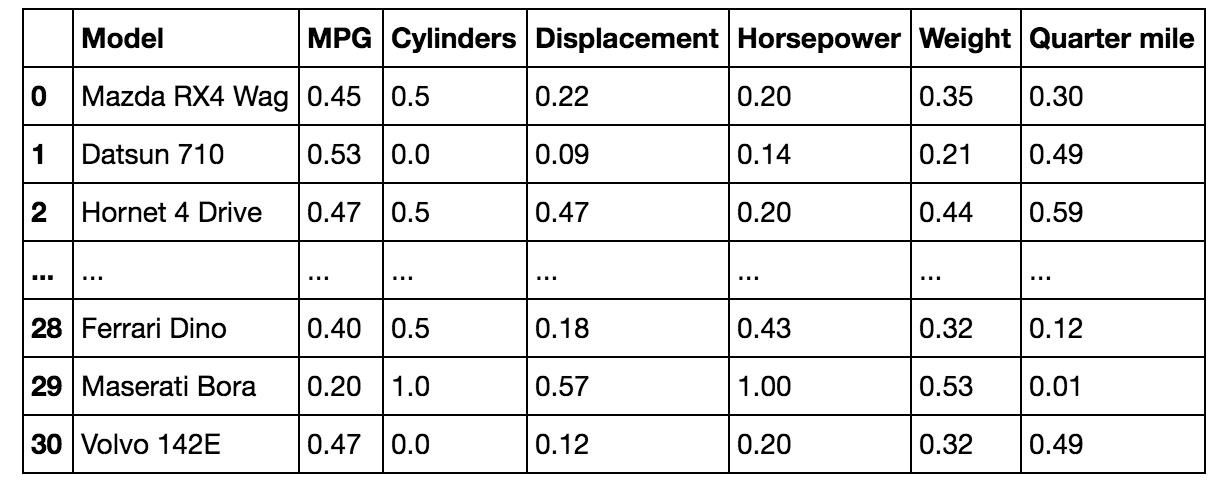
\includegraphics[height=50mm]{./images/CarsScaled.png}
\caption[Screenshot of Motor Trend Car Road Tests dataset included with R.]{Data from Fig. \ref{cars_dataset} rescaled to $(0,1)$.}
\label{cars_dataset_scaled}
\end{figure}
% Rescale the one-hot data instead

\section{Datasets for Neural Networks}\label{datasets}

When we train a neural network, we update its parameters--its weights and biases--so that it can learn to do useful things. This is what our brains do when we learn, updating synaptic strengths in order to function more effectively. As we will see, for unsupervised learning, we take an input dataset and train it to pick up statistical features of the data. For supervised learning, we take ``target data'' or ``labeled data'' and use it to train a network to do some desired thing.\footnote{Note that the term ``label'' is associated specifically with classification tasks, where an input is sorted into one of a finite set of categories. Think of labeling images as cat vs. dog. But not all training tasks are like that; regression tasks for example associate inputs with real-valued targets. ``Target data''  is thus a more general term. However, the terminology of ``labeled data''  has become standard, and  is snappier than ``input-target dataset''. We will use both terminologies interchangeably.}
% Reference to classification / regression discussion once that's done
% Note clever tricks to get labels, like auto-regressive to predict next token (forward ref Elman and SRN discussion), or GANs where all you need is images, or first part of wiki article from the rest of it.

To support these tasks, we must define several standard types of datasets:
\begin{itemize}
\item \textbf{Input dataset}: each row contains an input vector that can be sent to a neural network. This idea is illustrated in Fig. \ref{data_inputs}.
\item \textbf{Output dataset}: each row contains an output vector that has been recorded from a neural network. These are also called ``predictions''. 
\item \textbf{Target dataset (labels)}: each row contains a target output vector we'd like a neural network to produce for a given input vector. The target dataset is a set of \emph{desired outputs}, a set of labels.
\item \textbf{Labeled dataset}: an input dataset and a corresponding target dataset. Note that the two datasets must have the same number of rows. This idea is illustrated in Fig. \ref{supervised_learning}.
\end{itemize}
Examples of each type of dataset are shown in Fig. \ref{datasetTypes}.
% Graph showing availability of data vs. labeled data. 

% Include standard labels, like x for inputs,  y for labels, $\hat{y}$ for predictions

An \glossary{input dataset} contains input vectors to be sent to the input nodes of a neural network. Each row of an input dataset is a point in the input space of a neural network. Input datasets are used for all kinds of learning tasks, supervised and unsupervised. 

An \glossary{output dataset} is \emph{generated} from an input dataset. We feed each row of the input dataset to a network and record the resulting output vector. Thus, an output dataset will have as many rows as the input dataset used to train it. The phrase ``output dataset'' is non-standard. Since these are often interpreted as predictions given a set of inputs, this table is sometimes referred to as a set  of ``predictions''. 

A \glossary{target dataset} contains the outputs we \emph{want} the network to produce. These can be thought of as desired outputs. These targets are also called ``labels'', for classification tasks, described below. We compare an output dataset with a target dataset to produce an error, discussed in chapter \extref{ch_supervised}. Like an output dataset, a target dataset will have as many rows as a corresponding input dataset. 

A \glossary{labeled dataset} (also \emph{labeled data} or \emph{input-target dataset}) is a concatenation of two tables, an input and a target dataset. We can represent this by simply concatenating the two datasets and separating them with double vertical lines, as in the right-most panel of Fig. \ref{datasetTypes}. This is perhaps the most common type of dataset to consider, since it is a specification of a supervised learning task. Labeled data is often difficult to obtain, because we can't simply gather it ``from the world.''  If we take a bunch of pictures of people's faces and transform the data then we have our input dataset. But it is an extra step for a human to come in and label each face as male or female, so that we can confirm that a machine can also do the job. The contrast to labeled  data  is an input dataset by itself, or what is sometimes referred to as ``unlabeled data''. 

\begin{figure}[h]
\centering
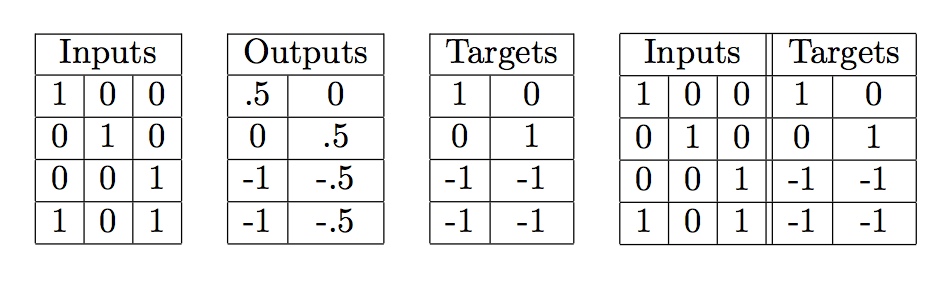
\includegraphics[width=0.7\textwidth]{./images/datasetTypes.png}
\caption[Jeff Yoshimi.]{From left to right: an input dataset, output dataset, target dataset, and labeled dataset.}
\label{datasetTypes}
\end{figure}

\section{Generalization and Testing Data }\label{generalization}

% Mention car network from videos and how we can train it then use it to predict new data
One attractive feature of neural networks is that even if they have been trained on a specific dataset, they will tend to generalize well to new patterns they weren't trained on. This is easy to see with the 3-object detector in Simbrain, discussed in section \extref{intro_comp_nn}. Try plugging in inputs it has not seen before, and it will still do well. This is a psychologically realistic property of neural networks. Suppose I have only ever seen two pineapples. My neural network was trained on only two pineapples. But I manage to correctly classify many other pineapples that I've never seen, even though they produce slightly different patterns on my eye. Our neural networks are good at \glossary{generalization}, at extrapolating from what they have seen to new things they have not seen.

% Mention relevant psychology studies below
On the other hand, sometimes the specific inputs a neural network is trained on are, in a sense, \emph{too} specific. Ideally, we have diverse inputs that allow us to deal well with new situations. But sometimes people are exposed to  data that is narrow and that leads to poor generalization. If you grow up in the forest you will be very good at classifying trees but not so good at classifying buildings. This is the origin of biases and stereotypes and linguistic accents. 

% Underfitting. Bias variance tradeoff. Glossary below, at least for overfitting.
This issue also comes up in neural networks. When you train a network on a labeled dataset, it can learn to be very good at predicting the target data you provide it. However, it might end up being \emph{too} finely tuned on that data and thus fail to do well with new data. This is called \emph{overfitting}. We want to build models that are not overfit to the data they were trained on. We want them to do well not just on the data we trained them on, but also on new data they have never seen. How well does the network generalize to new data?  This is also referred to as ``out of sample'' performance (how well does a model do outside of the same data it was trained on). We train a network on 30 cars, and then test it on a new car it's never seen before. Or we train a network to classify 100 letters, but then we give it new letters it's never seen before. A good network can generalize from what it's been trained on, to new data.

To deal with this issue, we partition a labeled dataset into two subsets. We train the network on one subset of data and then test it on another set of data that we have ``held out'' to see how well the network generalizes. These two subsets are a training subset and a testing subset of a labeled dataset.

A \glossary{training subset} or \emph{training dataset} or \emph{training data} is a subset of a labeled dataset used for training your model.

A  \glossary{testing subset} or \emph{testing dataset} or \emph{testing data} is a subset of a labeled dataset used for testing your model on new inputs. This is data that is held out to see how well a model generalizes. 

The idea is illustrated in Fig. \ref{trainTest}. The idea is that we first train the network using training data, and then validate it using testing data.\footnote{In a machine learning context, we might also distinguish working from production data. Working data includes all the data mentioned above, used to train and test and validate a machine learning model. Production data is then data the machine learning model encounters in the ``real world'' when it has been deployed and is being used.} 

\begin{figure}[h]
\centering
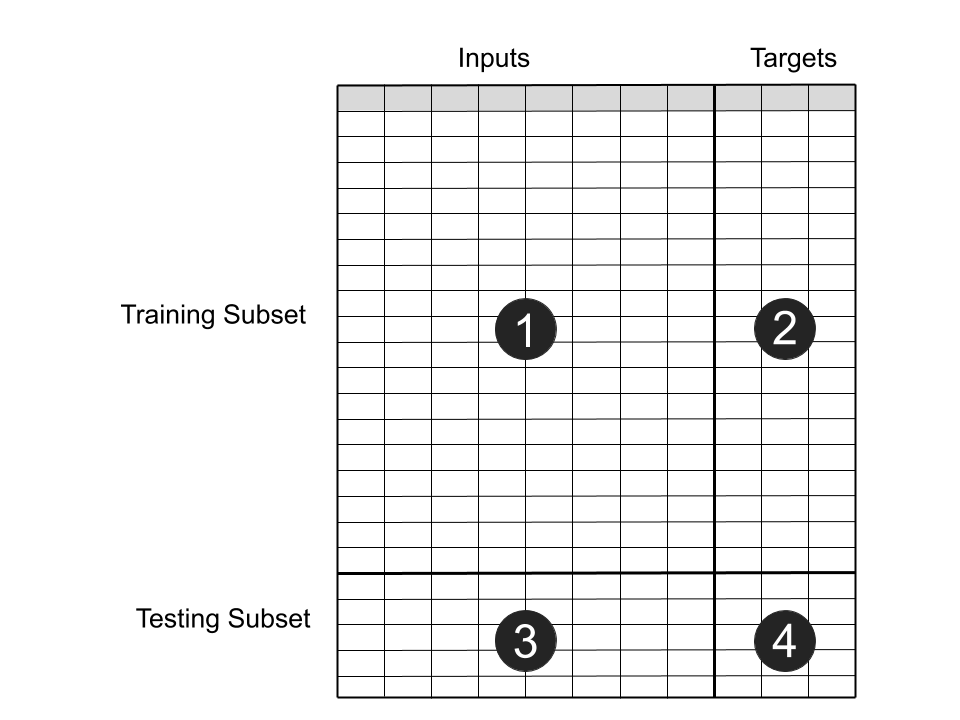
\includegraphics[scale=0.3]{./images/trainTest2.png}
\caption[Jeff Yoshimi.]{The rows of a labeled dataset (with inputs and targets) divided into a training and a  testing subset. The training subset is used to train our model, and the testing subset is used to validate how well it generalizes. Thus we end up with four tables: (1) training inputs, (2)  training targets or labels, (3) testing inputs, and (4) testing targets. }
\label{trainTest}
\end{figure}

So what we actually often end up with, in supervised learning, is four tables. (1) Training inputs, (2) test inputs, (3) training targets, and (4) test targets. The training inputs and targets are used to train the model. The test inputs and targets are used to determine how well it performs on new data. In a model we might label these \code{train\_inputs}, \code{train\_targets}, \code{test\_inputs}, and \code{test\_targets}. 

% Expand on batches
In practice, even more complex ways of partitioning labeled data into training and testing subset are used, for example splitting the data into training and testing sets different ways on different passes.\footnote{The more general topic is cross validation, see \url{https://en.wikipedia.org/wiki/Cross-validation_(statistics)} and \url{http://scikit-learn.org/stable/modules/cross_validation.html}.} The particular training subset used in a given stage of training is often referred to as a ``batch''. We are keeping things simple here for illustrative purposes.
 
% There is much more to say about this topic. In particular, when a neural network or other model overfits--performing well on the training subset but poorly on the testing subset--\emph{regularlization} methods are used to address the problem.\footnote{See \url{http://neuralnetworksanddeeplearning.com/chap3.html}} But we will not discuss these topics further here.

\section{Supervised vs. Unsupervised Learning}

% Add semi-supervised

We can distinguish two general ways of training a feed-forward neural network: supervised methods, where we tell the network what it should do with each input, and unsupervised methods, where we don't tell the network what we want it to do, but it figures out on its own (without a ``supervisor'') what to do. These concepts apply to recurrent networks as well, but we'll focus on feed-forward networks for now.

\begin{figure}[h]
\centering
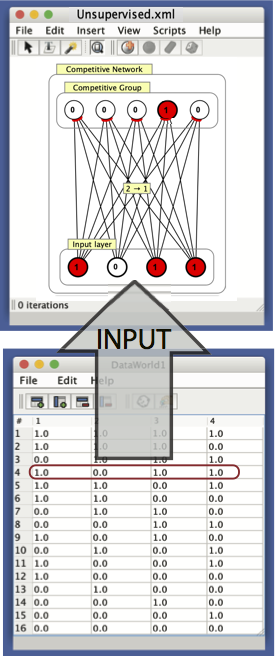
\includegraphics[width=0.2\textwidth]{./images/dataset_unsupervised.png}
\caption[Simbrain screenshot with graphical elements added by Pamela Payne.]{Illustration of how unsupervised learning relies only on an input dataset.}
\label{unsupervised_learning}
\end{figure}
% TODO: Clean up figure (which was hacked together) and use continuous valued inputs.

\glossary{Unsupervised learning}  is learning without a teacher, which is covered in chapters \extref{ch_unsupervised} and \extref{ch_unsupervised_recurrent}. We don't tell the network what we want. It must adapt on its own, discovering statistical patterns in the inputs it is exposed to. There is just an input dataset, as shown in figure \ref{unsupervised_learning}. There is no target data.  In the example shown in the figure, we repeatedly expose the network to a set of inputs, and it will automatically develop feature detectors, which respond to specific clusters in the input dataset.

This is  more neurally and psychologically realistic. After all, humans and animals don't constantly have a parent or teacher around telling them what's right or wrong.  For this reason we saw that it was a general principle of learning in the neuroscience chapter \extref{ch_neuro}. It is well known in psychology that a great deal of learning (e.g. ``latent learning'') occurs without explicit supervision; rats get to know their way around a maze even without explicit rewards \cite{wang2021latent}. It can also be useful in  machine learning, since we oftentimes don't have training data available (hence the term ``unlabeled data''). 

\begin{figure}[h]
\centering
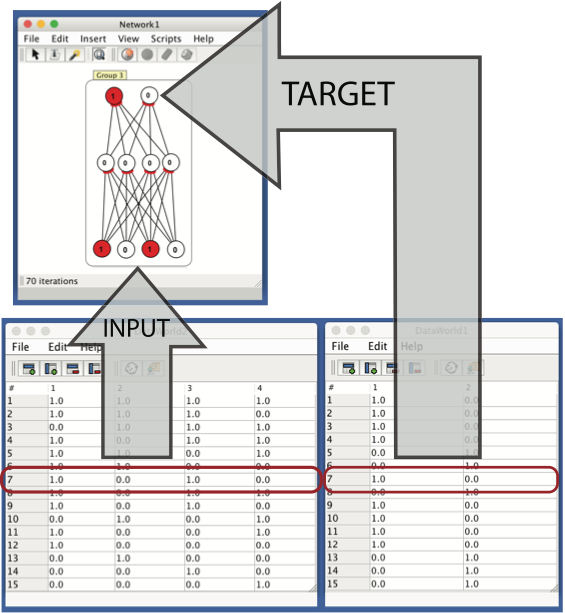
\includegraphics[width=0.4\textwidth]{./images/dataset_supervised.png}
\caption[Simbrain screenshot with graphical elements added by Pamela Payne.]{Illustration of how supervised learning uses both input and target datasets.}
\label{supervised_learning}
\end{figure}

In the case of \glossary{supervised learning}, we tell the network what we want it to do. There is a teacher or trainer and so we have a labeled dataset. It's kind of like a parent telling a child, ``No, that's wrong, this should be the answer!'' For feed-forward networks, this means we give it a labeled dataset and say ``implement that''! We train the network to perform a set of input-output associations. The general schema is illustrated in figure \ref{supervised_learning}. We train a network using a supervised learning algorithm using a labeled dataset, which includes \emph{two} tables, one for the inputs (the input dataset), and another for the outputs that we \emph{should} get for each input (the target dataset). As each row of an input dataset is  fed to the network, a corresponding row of a target dataset is used to determine how the network should respond. 

Supervised learning is a huge topic that will be covered in chapter \extref{ch_supervised}. Almost all of the major examples of things neural networks have done--drive cars, classify letters, translate languages or speech signals, etc. (see chapter \extref{ch_intro})--were achieved using supervised learning. However these methods are not just useful in engineering. They have also been used to used in connectionism and computational cognitive neuroscience to study the kinds  of representations the brain develops based on its exposure to inputs. Recall, for example, the discussion of the cerebellum and basal ganglia in chapter \extref{ch_neuro}, both of which are thought to learn via supervised learning.

\section{Other types of model and learning algorithm}

Learning algorithms and the models they are used to train can be classified in other ways as well. For example, in chapter \extref{ch_supervised_ff} we distinguish between supervised learning models that peform \glossary{classification task}s and \glossary{regression task}s, which is based on whether the target dataset contains categorical one-hot data (classification) or real-valued numerical data (regression).  

Another distinction that is sometimes useful is that between a \glossary{generative model} and a \glossary{discriminative model}. A generative model is a model that can be used to generate prototypical features of a category with a given category label. They can be feed-forward networks that associate one-hot localist vectors with distributed feature vectors. For example, if you are asked to ``describe a typical Golden Retriever'', or ``what are the height and weight of an average third grader'', you can generate answers. These are contrasted with \glossary{discriminative model}s, where features are associated with categories. For example, if you are shown a picture of a dog and asked ``is this a Golden retriever?'', or a picture of a person and asked ``is this a third grader?'', you are simply discriminating a category based on inputs.  A discriminative model is less demanding than a generative model, since you only must categorize items, rather than generating examples of items from a category (Compare multiple-choice questions with fill-in-blank questions on a test. Fill in the blank is harder, because you must generate and answer rather than just recognizing one answer as correct). Discriminative models, like classifiers (see chapter \extref{ch_supervised_ff}), are the focus of much of this book, and are well known in machine learning. Face and text recognition are usually based on discriminative models.  But generative models are also important. For example, models that generate human speech or fake text are discussed in chapter \extref{ch_supervised_recurrent}.\footnote{I am using non-standard and informal definitions of generative and discriminative models. A generative model is formally defined as a model of the joint probability distribution over inputs and outputs of a model, where the outputs are often categorical, which means that given a category you can estimate the associated features. A discriminative model is defined as a model of the probability of outputs given inputs.} 

There are other types of learning algorithms and approaches to learning in neural networks as well.

An \glossary{evolutionary algorithm} (or genetic algorithm) is a class of algorithm that simulate evolutionary processes. You start by saying what counts as fitness and then set up an array of simulated genes and some kind of simulation. Then you run it!  Millions of years of evolution can be compressed into minutes of time, as millions of simulations are run. When applied to neural networks, a batch of networks can be built, based on incrementally varying and mutated genes. The best are selected and further permuted, and the process continues. The script \emph{evolveNetwork.bsh} in Simbrain evolves a network such that on average half of the nodes are active every few iterations. Run it a few times. You will see that it evolves a variety of solutions to the problem.

% Mention dopamine and basal ganglia below; a link  to the neuroscience chapter
% Sharai - Skinner wrote several different books on behaviorism, of which there are multiple editions. Which do we use for reference?
Another approach to training, \glossary{reinforcement learning}, is a variant of supervised learning where you don't just give the network a table of values to associate, but rather the action of an agent in a simulated environment, which tells the network when what it's doing is good or bad. This is a kind of virtual implementation of behaviorist psychology (Skinner famously thought all behavior could be explained as the result of a history of reinforcement and punishment). So you take a virtual agent, put it in a virtual environment, and tell it what  is good and bad in that environment. Getting the cheese is good. Getting attacked is bad. Now you simulate thousands or millions of explorations of the environment and it will learn to approach cheese and avoid predators. Some of the major recent developments in machine learning have been based on reinforcement learning (e.g. the success of AlphaGo) \cite{silver2016mastering}. Another famous example is a system that learned to play a bunch of old Atari video games \cite{mnih2013playing}. The nice thing about reinforcement learning is that it is fairly realistic. As noted in chapter \extref{ch_neuro}, the basal ganglia are thought to mediate a form of reinforcement learning such that animals learn to maximize reward over time. 
% We will see a detailed model along these lines in the chapter on basal ganglia.

There are yet other methods, and machine learning is constantly evolving and adding more techniques and learning algorithms to its roster of approaches. 

 %Time series methods
% Stability / Plasticity / artnets
% Bayesian techniques. Active Learning.
% Boltzman machines?
